%! Tex program = xelatex   
\documentclass{article}
\usepackage{graphicx,subfig}
\usepackage[left=2cm, right=2cm, lines=45, top=0.8in, bottom=0.7in]{geometry}
\usepackage{xeCJK}
\usepackage{amsmath}
\usepackage{booktabs} %表格
\usepackage{tikz}
\usepackage{graphics}
\usepackage{xcolor} 
\usepackage{tikz} 
\usepackage{svg}
\usetikzlibrary{arrows,shapes,chains}
\setmainfont{Times New Roman}
\setCJKmainfont{Songti SC}
\setCJKfamilyfont{song}{Songti SC}
\renewcommand{\baselinestretch}{1.5} %行间距
%-----------------------伪代码------------------
\usepackage{algorithm}  
\usepackage{algorithmicx}  
\usepackage{algpseudocode}  
\floatname{algorithm}{Algorithm}  
\renewcommand{\algorithmicrequire}{\textbf{Input:}}  
\renewcommand{\algorithmicensure}{\textbf{Output:}} 
\usepackage{lipsum}  
\makeatletter
\newenvironment{breakablealgorithm}
  {% \begin{breakablealgorithm}
  \begin{center}
     \refstepcounter{algorithm}% New algorithm
     \hrule height.8pt depth0pt \kern2pt% \@fs@pre for \@fs@ruled
     \renewcommand{\caption}[2][\relax]{% Make a new \caption
      {\raggedright\textbf{\ALG@name~\thealgorithm} ##2\par}%
      \ifx\relax##1\relax % #1 is \relax
         \addcontentsline{loa}{algorithm}{\protect\numberline{\thealgorithm}##2}%
      \else % #1 is not \relax
         \addcontentsline{loa}{algorithm}{\protect\numberline{\thealgorithm}##1}%
      \fi
      \kern2pt\hrule\kern2pt
     }
  }{% \end{breakablealgorithm}
     \kern2pt\hrule\relax% \@fs@post for \@fs@ruled
  \end{center}
  }
\makeatother
%------------------------代码-------------------
\usepackage{xcolor} 
\usepackage{listings} 
\usepackage{fontspec}
\newfontfamily\menlo{Menlo}
\setmonofont[Mapping={}]{Monaco} 
\definecolor{mygreen}{rgb}{0,0.6,0}
\definecolor{mygray}{rgb}{0.5,0.5,0.5}
\definecolor{mymauve}{rgb}{0.58,0,0.82}
\lstset{ %
backgroundcolor=\color{white},   % choose the background color
basicstyle=\footnotesize\ttfamily,        % size of fonts used for the code
columns=fullflexible,
breaklines=true,                 % automatic line breaking only at whitespace
captionpos=b,                    % sets the caption-position to bottom
tabsize=4,
commentstyle=\color{mygreen},    % comment style
escapeinside={\%*}{*)},          % if you want to add LaTeX within your code
keywordstyle=\color{blue},       % keyword style
stringstyle=\color{mymauve}\ttfamily,     % string literal style
frame=single,
rulesepcolor=\color{red!20!green!20!blue!20},
numbers=left,
 numberstyle=\tiny\menlo
% identifierstyle=\color{red},
% language=c++,
}
\begin{document}
\title{核酸检测登记系统}
\author{朱浩泽 1911530 \ \ \ 何坤彬 1911417}
\maketitle
\section{软件需求和设计}
\large
\subsection{需求背景}
2020年伊始,一场突如其来的新型冠状病毒肺炎疫情,在春节期间突袭神州大地,面对困难,举国上下团结一心,共同投入到抗击疫情的工作中。在党中央坚强领导下,中国人民风雨同舟、众志成城,发扬一方有难、八方支援精神,构筑起疫情防控的坚固防线。广大医务人员白衣为甲、逆行出征,为保障人民的健康,进行了一轮又一轮的健康监测。而这些检测结果的数据量是庞大的,这就需要我们对海量的信息进行有效的组织管理,来确保信息的准确性和完整性。于是,我们计划开发一款核酸检测登记系统。
\subsection{系统设计思路}
\ \ \ \ \ 在拥有需求之后,我们可以对我们的系统进行设计。首先,核酸登记系统需要识别被登记人,而如果用人名作为登记人员的信息,可能会有很多重名的人员导致信息混乱。所以我们需要选取每个人都具有的且为独一无二的表示方式。在现如今的社会,每个人都拥有着自己的身份证号,且是一人一号,具有问一下。由此可见身份证号可以很好的承载着我们的需求,故选取身份证号作为登记人员的身份标识,配合被测人员的姓名进行辅助。

接下来便是,当我们获得了人员的信息后,需要存储其核酸检测状态,所以需要存储人员的检测情况(阴性/阳性)。在检测后,我们也要给被测人员一个检测情况的反应,并在必要时(万一呈现阳性时)可以找到被测人员,所以我们要记录被测人员的手机号以便进行联系和反馈,并登记被检测人员的住址进行潜在的流行病学调查。由于疫情发展瞬息万变,一个人可能会测多次核酸,所以我们还要记录其检测时间,以区分不同批次检测结果。而且,不同人群的身体反应可能也是不一样的,所以我们还要记录人员的年龄信息。所以我们。这里我们选择了一个简单的数据库,其中包含了人员的身份证号、姓名、检测状态(阴性/阳性)、检测时间、检测结果(阴性/阳性)。

当然,为了加快信息录入的速度,我们允许多人对信息进行登录。同时又避免信息的混乱和保证信息的安全性,我们采取了注册制度。用户需要先进行注册,然后医护人员才可以为用户的核酸检测数据进行上传和更改,由于核酸检测只有最近的结果是有说服性的,所以我们每次登记时只相当于更改被登记人的最后一次见的时间和检测记录。

我们采用java框架配合mysql数据库进行系统设计。
\section{系统实现方法}
\subsection{编程环境}
该核酸检测登记系统在Windows 64位的机器上使用java语言以及MySQL数据库实现。
\subsection{连接MySQL数据库}
该系统需要连接数据库nadrs,使用root权限,密码为123456:
\begin{center}
   \includegraphics*[scale = 0.5]{1.jpg}
\end{center}
\begin{lstlisting}[language = java]
   private static String driver = "com.mysql.jdbc.Driver";// 驱动程序名
	private static String URL = "jdbc:mysql://localhost:3306/nadrs?useSSL=false&allowPublicKeyRetrieval=true";// URL指向访问的数据库
	private static Connection con = null;
	private static Statement smt = null;
	private static ResultSet rs = null;

	private static Connection createConnection() {
		try {
			Class.forName(driver);// 加载驱动程序
			return DriverManager.getConnection(URL, "root", "123456");// 以root权限连接数据库
		} catch (SQLException e) {
			System.out.println(e.getMessage());
			e.printStackTrace();
		} catch (java.lang.ClassNotFoundException e) {
			e.printStackTrace();
			System.out.println("Can't load Driver");
		}
		return null;
	}
\end{lstlisting}

java提供连接数据库的包,通过加载"com.mysql.jdbc.Driver"驱动程序实现对数据库的连接。同时能够实现对数据库SQL语句的执行,我们将其封装为runUpdate、runBatch、runQuery函数以供操作数据库时调用:
\begin{lstlisting}[language = java]
   public static int runUpdate(String sql) throws SQLException {
		int count = 0;
		if (con == null) {
			con = createConnection();
		}
		if (smt == null) {
			smt = con.createStatement();
		}

		count = smt.executeUpdate(sql);

		if (smt != null) {
			smt.close();
			smt = null;
		}
		if (con != null) {
			con.close();
			con = null;
		}
		return count;
	}

	public static void runBatch(ArrayList<String> s) throws SQLException {
		if (con == null) {
			con = createConnection();
		}
		if (smt == null) {
			smt = con.createStatement();
		}
		for (int i = 0; i < s.size(); i++) {
			System.out.println(s.get(i));
			smt.addBatch(s.get(i));
		}
		smt.executeBatch();
		return;
	}

	public static ResultSet runQuery(String sql) throws SQLException {
		if (con == null) {
			con = createConnection();
		}
		if (smt == null) {
			smt = con.createStatement();
		}
		return smt.executeQuery(sql);
	}
\end{lstlisting}

\subsection{登录界面的实现}
登录界面需要使用到数据库中的user表,user表在数据库中结构为:
\begin{center}
   \includegraphics*[scale = 0.5]{2}
\end{center}

用户在文本框中输入用户名和密码,点击登录按钮后,程序会读取文本框中的内容,并且去数据库中查询uesr表中是否有对应的用户以及其对应的密码是否正确,若密码错误则登录失败。当然也可以点击注册按钮,程序会按照你输入的用户名和密码在user表中新添加一项记录,这样就可以使用该用户名和密码登录了,其登录和注册对应的java代码如下:

\begin{lstlisting}[language = java]
   @Override
	public boolean certifyUser(String uname, String upassword) {
		String select = "select * from user where uname='" + uname + "' and upassword='" + upassword + "'";
		boolean isCertifyUser = false;
		try {
			ResultSet rs = DBUtil.runQuery(select);
			if (rs != null) {
				isCertifyUser = rs.next();
				DBUtil.realeaseAll();
			}
		} catch (SQLException ex) {
			Logger.getLogger(UserDaoImp.class.getName()).log(Level.SEVERE, null, ex);
		}
		return isCertifyUser;
	}

	@Override
	public boolean addUser(User user) {
		String insert = "insert into user(uname,upassword) values('" + user.getUname() + "','" + user.getUpassword()
				+ "')";
		try {
			DBUtil.runUpdate(insert);
			return true;
		} catch (SQLException ex) {
			Logger.getLogger(UserDaoImp.class.getName()).log(Level.SEVERE, null, ex);
		}
		return false;
	}
\end{lstlisting}

\subsection{主界面实现}
主界面需要使用到数据库中的taker表,其结构如图所示:
\begin{center}
   \includegraphics*[scale = 0.5]{3}
\end{center}

程序通过getAllTaker函数获取数据库中taker表所有的内容,并通过java中JScrollPane将所有人员的信息展示在主界面上:
\begin{lstlisting}[language = java]
   @Override
	public List<NadTaker> getAllTaker() {
		String select = "select * from taker";
		try {
			List<NadTaker> takers = new ArrayList<NadTaker>();
			ResultSet rs = DBUtil.runQuery(select);
			while (rs.next()) {
				NadTaker taker = new NadTaker();
				taker.setSid(rs.getInt("sid"));
				taker.setSname(rs.getString("sname"));
				taker.setSnumber(rs.getString("snumber"));
				taker.setSage(rs.getInt("sage"));
				taker.setSphone(rs.getString("sphone"));
				taker.setSaddress(rs.getString("saddress"));
				taker.setState(rs.getString("state"));
				taker.setStime(rs.getString("stime"));
				takers.add(taker);
			}
			DBUtil.realeaseAll();
			return takers;
		} catch (SQLException ex) {
			Logger.getLogger(UserDaoImp.class.getName()).log(Level.SEVERE, null, ex);
		}
		return null;
	}
\end{lstlisting}

\subsection{检测人员注册功能实现}
在一个人进行检测之前首先需要将其身份信息登记进入系统中,这一功能在选择菜单中的登记按钮下实现,点击这一按钮会弹出登记界面,在文本框中输入对应内容后点击注册,系统会读取文本框中内容并在数据库的taker表中insert一条对应的记录。关键函数registerTaker代码如下:

\begin{lstlisting}[language = java]
   @Override
	public boolean registerTaker(NadTaker nadTaker) {
		String insert = "insert into taker(sname,snumber,sage,sphone,saddress,state,stime) " + "values('"
				+ nadTaker.getSname() + "','" + nadTaker.getSnumber() + "','" + nadTaker.getSage() + "','"
				+ nadTaker.getSphone() + "','" + nadTaker.getSaddress() + "','" + nadTaker.getState() + "','"
				+ nadTaker.getStime() + "')";

		try {
			// System.out.println(insert);
			DBUtil.runUpdate(insert);
			return true;
		} catch (SQLException ex) {
			Logger.getLogger(UserDaoImp.class.getName()).log(Level.SEVERE, null, ex);
		}
		return false;
	}
\end{lstlisting}

\subsection{检测人员登记功能实现}
我们可以通过点击选择菜单中的登记按钮对已经录入系统的人员进行核酸检测结果登记,在弹出的界面的文本框中输入其身份证号和检测时间、检测结果后,系统会读取文本框中的内容,执行checkNadTaker函数对user表中对应身份证号的记录进行核酸检测时间和核酸检测结果的更新:

\begin{lstlisting}[language = java]
   @Override
	public boolean checkNadTaker(String number, String time, String res) {
		String select = "select * from taker where snumber='" + number + "'";
		try {
			ResultSet rs = DBUtil.runQuery(select);
			if (rs.next()) {
				String update = "update taker set stime='" + time + "', state='" + res + "' where snumber='" + number
						+ "'";
				DBUtil.runUpdate(update);
				return true;
			}

		} catch (SQLException ex) {
			Logger.getLogger(UserDaoImp.class.getName()).log(Level.SEVERE, null, ex);
		}
		return false;
	}
\end{lstlisting}

\subsection{查询功能实现}
点击选择菜单中的查询按钮,在弹出的界面的文本框中输入需要查询的身份证号后点击查询按钮,系统会读取你输入的身份证号后在数据库的taker表中进行查询并返回对应的核酸检测结果:

\begin{lstlisting}[language = java]
   @Override
	public String getAnswer(String number) {
		String select = "select state from taker where snumber='" + number + "'";
		try {
			ResultSet rs = DBUtil.runQuery(select);
			while (rs.next()) {
				return rs.getString("state");
			}

		} catch (SQLException ex) {
			Logger.getLogger(UserDaoImp.class.getName()).log(Level.SEVERE, null, ex);
		}
		return "查无此人";
	}
\end{lstlisting}

\section{用户界面交互展示}
\subsection{登录}
\begin{center}

\includegraphics[width=0.5\textwidth]{图片/1}
\includegraphics*[width=0.5\textwidth]{图片/2}
\end{center}
\subsection{登录后的界面}
\begin{center}
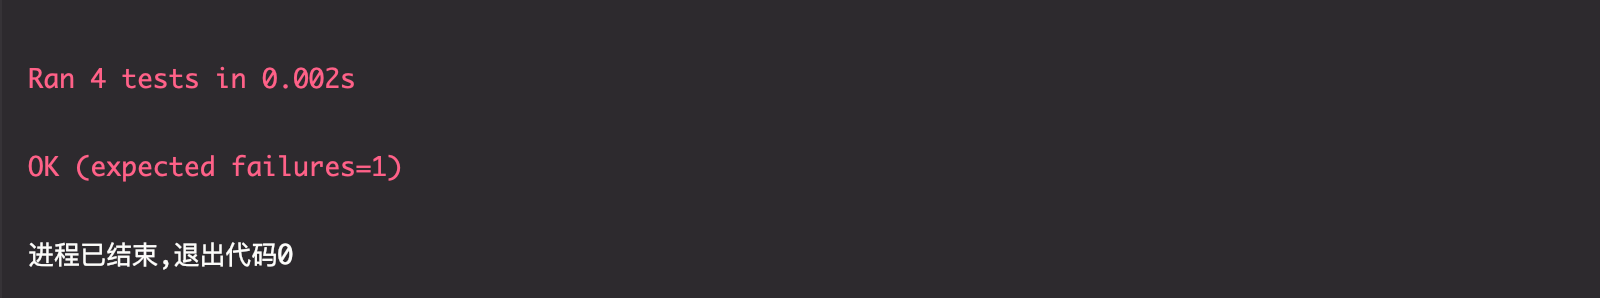
\includegraphics[width=0.5\textwidth]{图片/3}
\end{center}
\subsection{用户注册}
\begin{center}
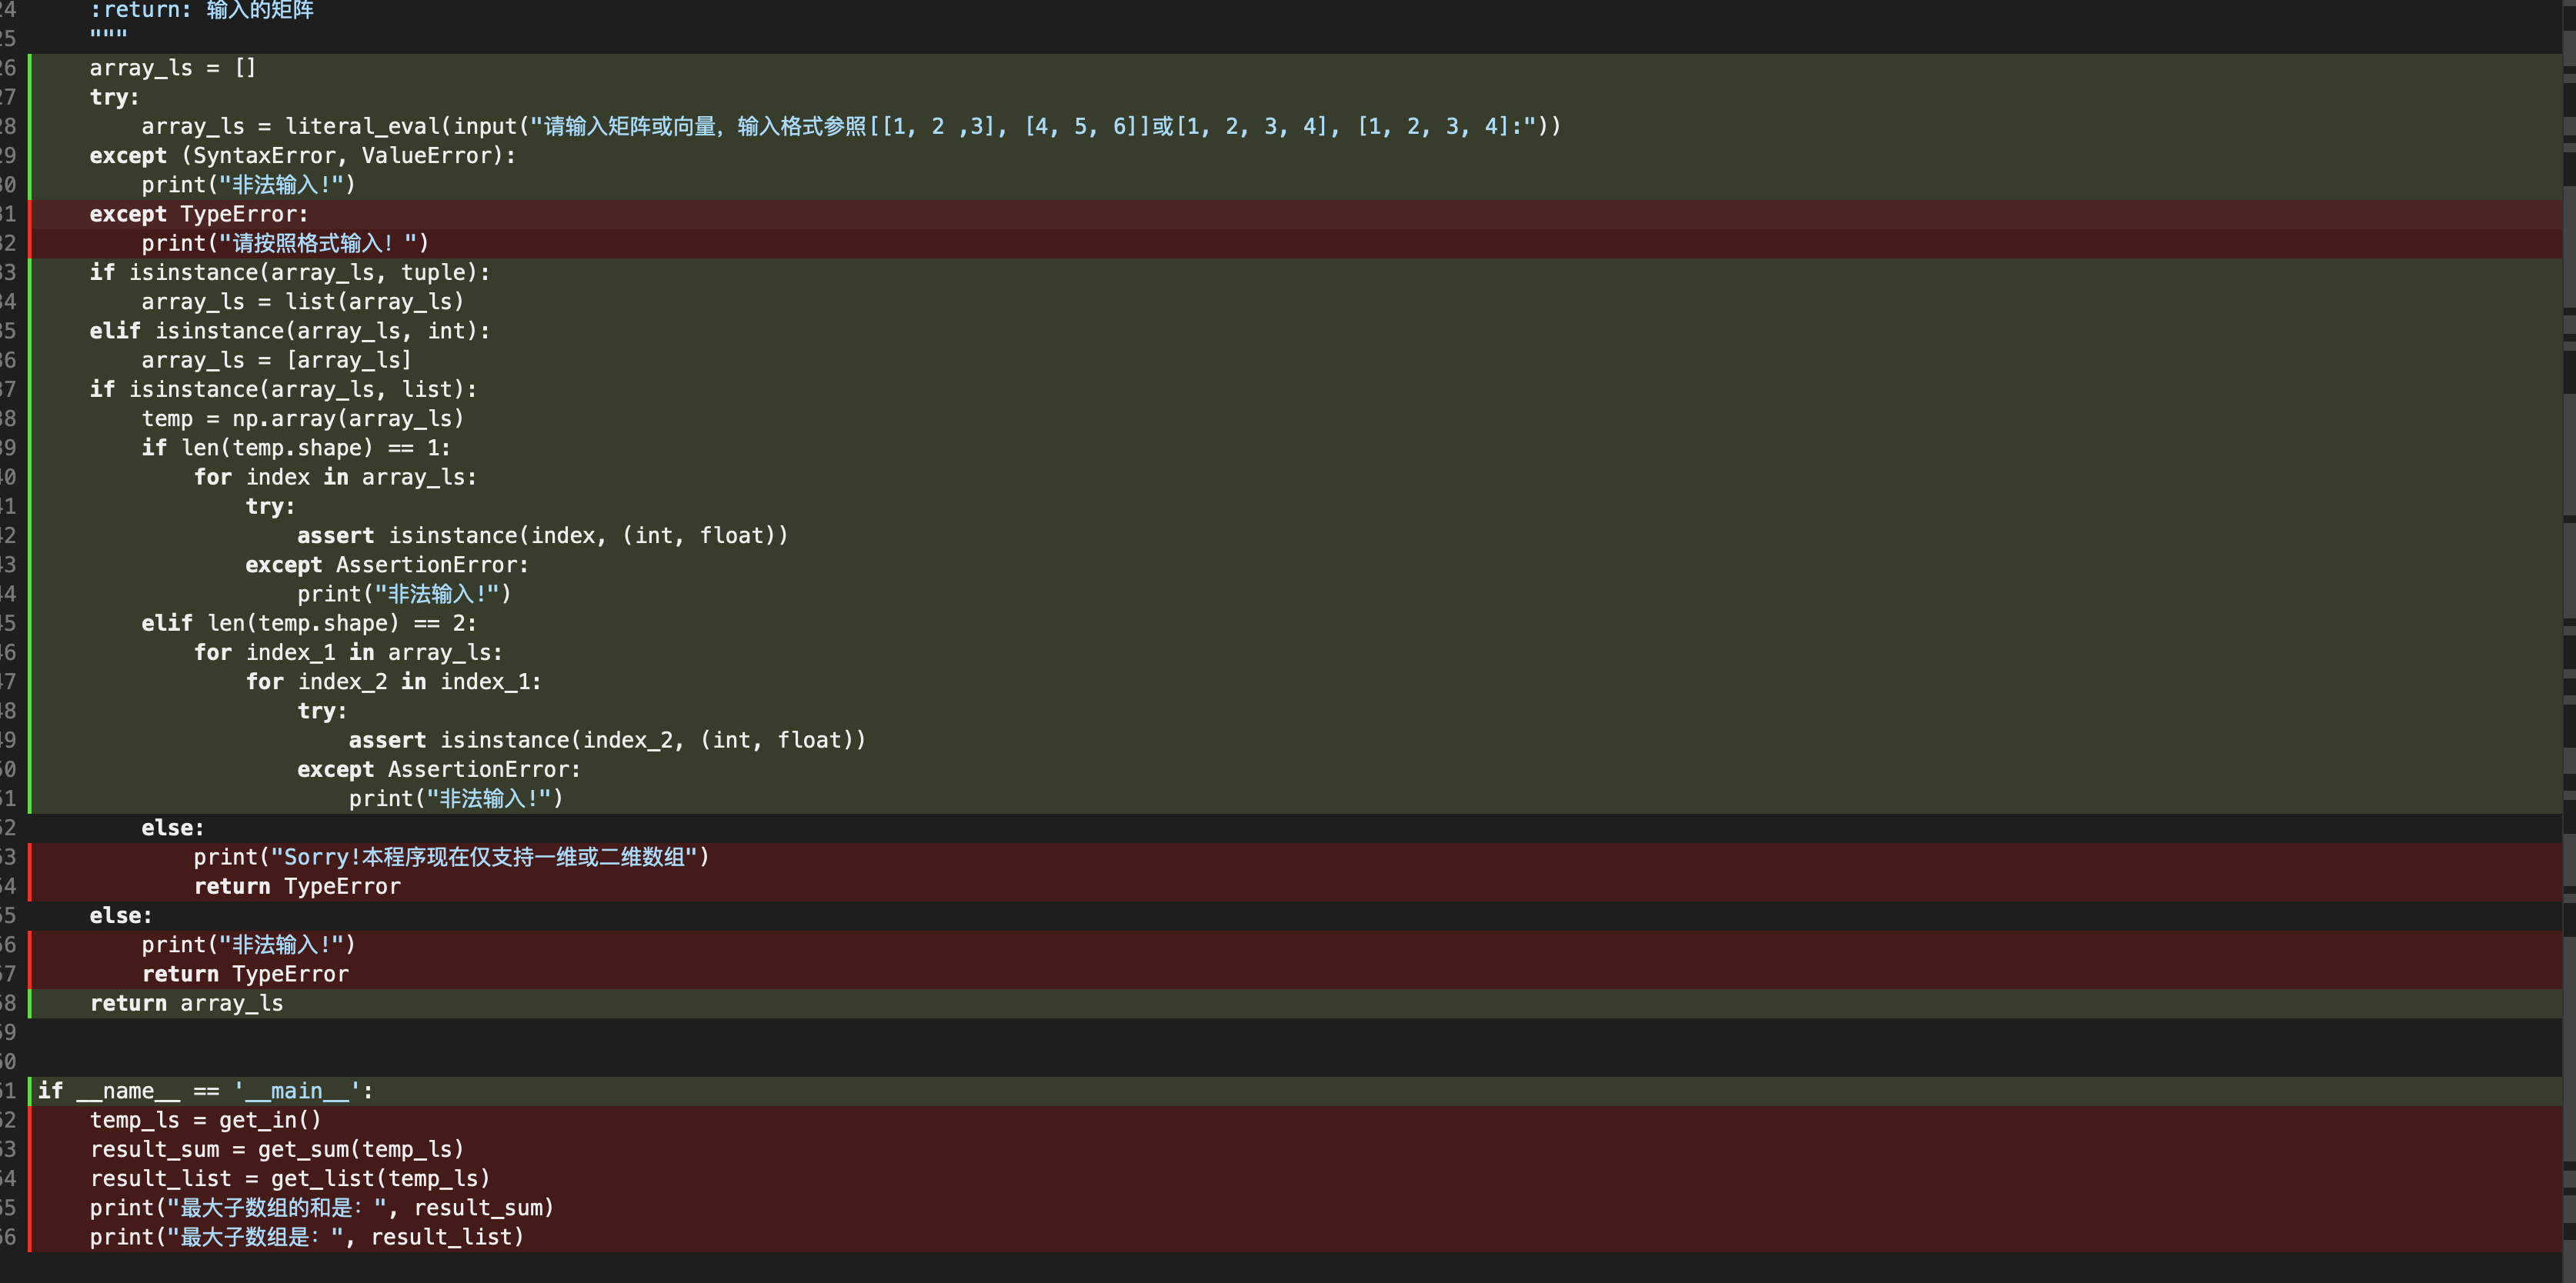
\includegraphics[width=0.5\textwidth]{图片/4}
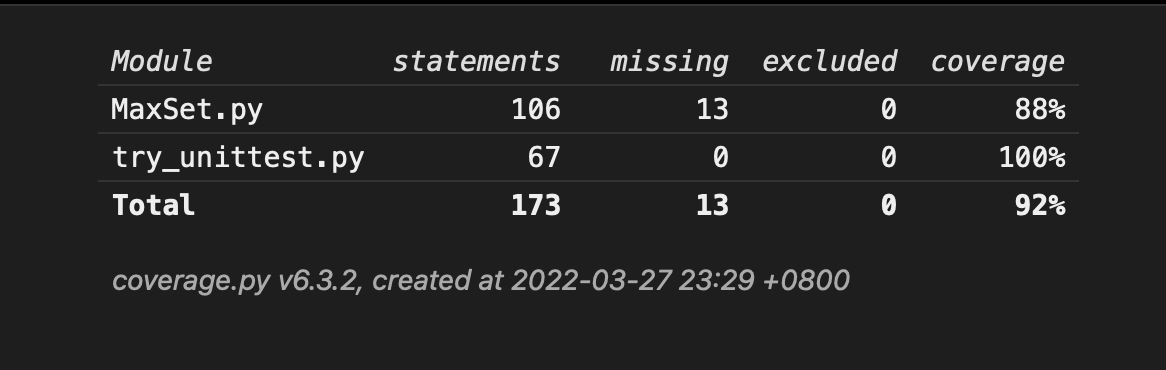
\includegraphics[width=0.5\textwidth]{图片/5}
\includegraphics[width=0.5\textwidth]{图片/6}
\end{center}
注册成功后刷新便可以看到人员信息
\begin{center}
\includegraphics[width=0.5\textwidth]{图片/7}
\includegraphics[width=0.5\textwidth]{图片/8}
\end{center}
\subsection{查询}
\begin{center}
\includegraphics[width=0.5\textwidth]{图片/9}
\includegraphics[width=0.5\textwidth]{图片/10}
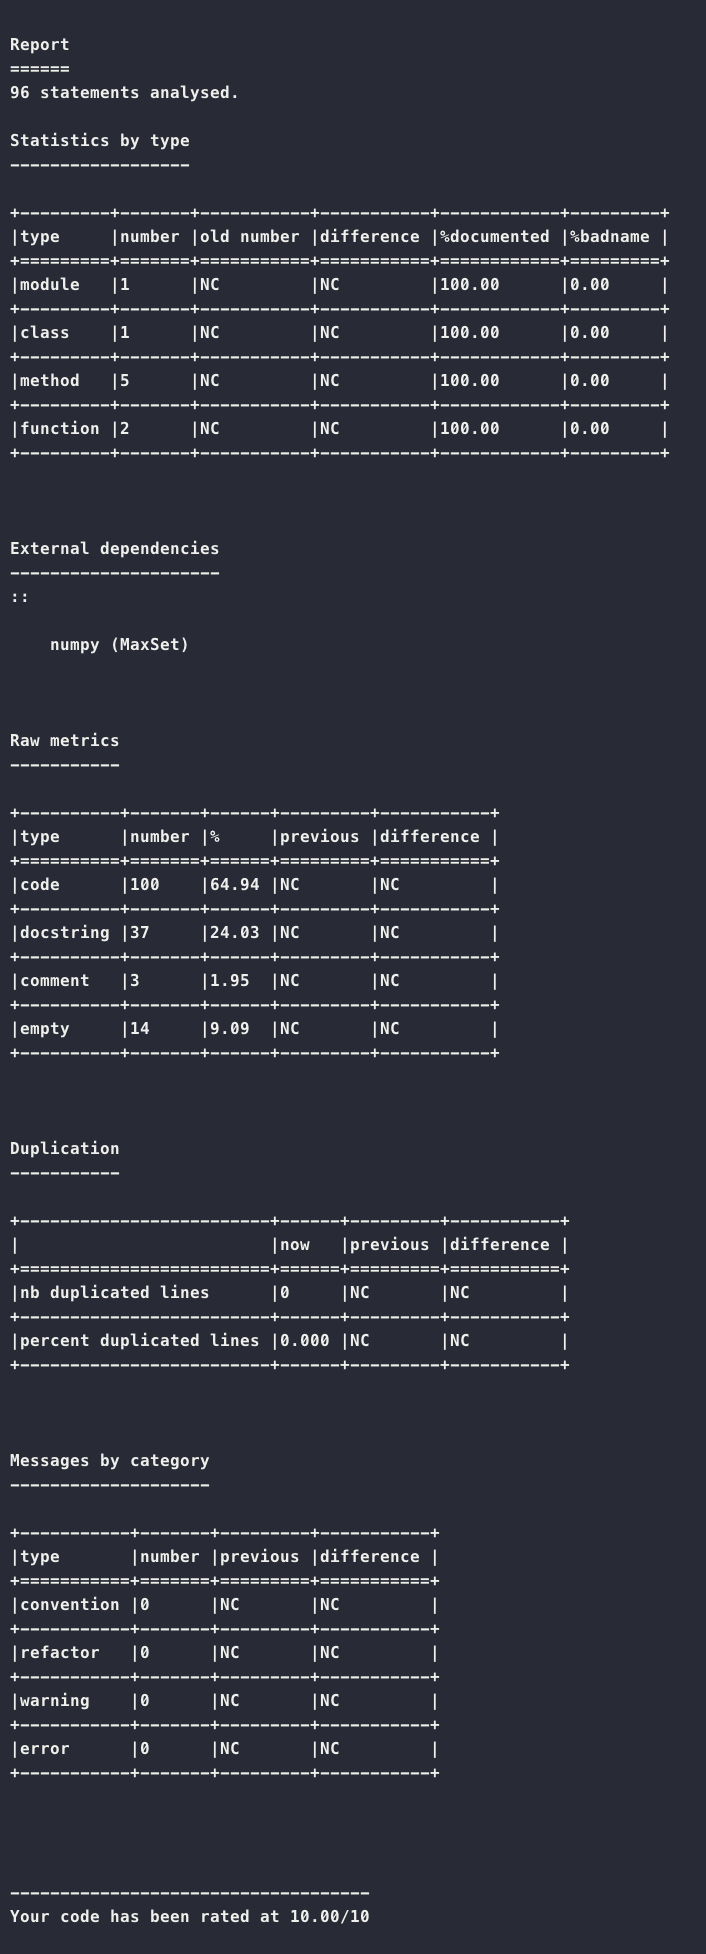
\includegraphics[width=0.5\textwidth]{图片/11}
\includegraphics[width=0.5\textwidth]{图片/12}
\includegraphics[width=0.5\textwidth]{图片/13}
\end{center}
\subsection{登记检测结果}
\begin{center}
\includegraphics[width=0.5\textwidth]{图片/14}
\includegraphics[width=0.5\textwidth]{图片/16}
\includegraphics[width=0.5\textwidth]{图片/17}
\includegraphics[width=0.5\textwidth]{图片/18}
\end{center}

刷新后可以看到新登记的检测结果

\begin{center}
\includegraphics[width=0.5\textwidth]{图片/19}
\includegraphics[width=0.5\textwidth]{图片/20}
\includegraphics[width=0.5\textwidth]{图片/21}
\includegraphics[width=0.5\textwidth]{图片/22}
\end{center}
\section{角色轮换安排}
我们的角色轮换较为明确,在编写数据库和设计数据库和java编程的后端这两部分时,由何坤彬充当领航员,朱浩泽充当驾驶员;在进行java部分的可视化操作的前端部分由朱浩泽充当领航员,何坤彬充当驾驶员。
\section{代码复审及讨论改进的过程}
\ \ \ \ \ 在最初,我们设计的mysql表非常简单,只有一个检测结果表(身份证号,姓名,检测结果)和一个用户表(用户名,密码),但此时领航员立刻指出,这样无法将用户表和检测结果表关联起来,所以增加了用户id这一特征将两张表中的内容进行关联。

随后,领航员又一次指出,这样设计的功能过于薄弱,核酸检测结果可能随时需要更新,所以又增加了检测时间这一特征,将检测结果和检测时间关联起来。随后,又考虑到溯源和通知的问题,我们又加入了被测人的家庭住址和联系方式,方便进行通知和溯源工作。

在进行java编程时,领航员随时关注着驾驶员的操作进度,驾驶员每次操作完成后,领航员会提醒他,并且提供一个操作完成后的提示,这样驾驶员就可以更加清晰的了解自己的操作进度。每次驾驶员编写代码时,领航员根据功能指挥驾驶员添加注释信息等,并按照代码规范对驾驶员进行变量命名的提示,每完成一个模块,驾驶员都要对代码进行测试,测试代码的正确性。领航员在每次驾驶员编写完代码进行测试后,对领航员编写的代码进行规范性检查,检查代码的编写规范,并且提供代码的检查结果。在这里,我们选取alibaba开发的Alibaba Java Coding Guidelines插件对代码的规范性进行检查,我们在类名处点击右键,可以看到“编码规约扫描选项”,根据该选项,领航员对代码的规范性和可读性进行检查,并在第一时间对不规范的代码进行正确的修改。领航员在这时候也可以看出驾驶员的代码编写习惯,并将在后面的编写过程中对驾驶员的糟糕编写习惯进行提醒。代码规范性和可读性检查如下:\textbf{(在这里,我们对大括号进行了要求,像if这种的条件判断和for这种的循环语句,无论接下来的代码块是一行还是多行的代码,一律都被大括号括起来)}

\begin{center}
	\includegraphics*[scale = 0.25]{截屏2022-04-25 16.53.45.png}
\end{center}

接下来,领航员应当对代码的覆盖率进行复审,

然后,领航员要考虑代码的可读性,假设自己是一个于此项目不相关的人员





\section{双人合作的工作照片}
\centerline{\includegraphics[width=0.5\textwidth]{IMG_1532.JPG}}
\section{对方编程习惯总结和性格评价}
\section{心得体会}
\end{document}
